% Einf�hrung - l�schen!

%\emph{Dieses Dokument soll eine grobe, nicht notwendigerweise vollst�ndige Richtlinie darstellen, auf welche Punkte beim Durchlesen
%des Artikels geachtet werden sollte. Manche Punkte oder Abschnitte treffen eventuell auf den Artikel nicht zu oder lassen sich besser
%in einer anderen Reihenfolge erkl�ren. F�r die Ausarbeitung ist es deshalb notwendig, eine Auswahl
%der wichtigsten Punkte zu treffen, die dann im Text in einen sinnvollen Zusammenhang gebracht werden.
%Die �berschriften k�nnen f�r die Ausarbeitung �bernommen werden, die Aufz�hlungen sollen aber
%durch zusammenh�ngenden Text ersetzt werden. Insgesamt maximal vier, besser drei Seiten.
%}

% Haupttext

\begin{abstract}
	

\end{abstract}

\section{Reinforcement learning method and regression model }

We chose Q-learning as reinforcement learning method, and we try to use two different regression models, Neural network and regression forest.   

\subsection{Q-learning }
In Q-learning we define a function $Q(s,a)$ representing the discounted future reward when we perform action $a$ in state $s$, and continue optimally from that point on.

$Q(s_t,a_t)=max_{\pi}R_{t+1}$
\newline
Where $R_{t+1}$ represents the total future reward at step $t+1$ and
$\pi$ is the policy, the rule how we choose an action in each state.
\newline
The way to think about $Q(s,a)$ is that it is "the best possible score at the end of game after performing action $a$ in state $s$". It is called Q-function, because it represents the "quality" of certain action in given state.

Let?s focus on just one transition $(s,a,r,s')$. Just like with discounted future rewards in previous section we can express Q-value of state $s$ and action $a$ in terms of Q-value of next state $s'$.



\subsection{Neural Network as regression model}

\subsection{Regression forest as regression model}

\subsection{First attemp approach}
In order to construct the states, we found three set of crucial parameters to describe the situations in the game.
The first set, related to the avaliable cells to move, is constructed by means of an array of four boleans.
\subsection{States construction:}
\subsubsection{Avaliable cells array (ACA)}
\label{section:ACA}
The first set, a boolean one, provides the information of the available cells surrounding the agent. If a bit is on, that means this direction is free to move.
We provide some examples for better understanding, the first column indicates the available moves, the second the abbreviation of the direction and the third one the related set. Showed in the next table \ref{table:S1}:

\begin{center}
    \captionof{table}{Avalible moves, abbreviation and related boolean array.}
  \begin{tabular}{|l|c|c|}
\hline
Avalible moves & Abbreviation & First set examples \\ \hline
Up          & $U$ & $(1,0,0,0)$ \\
Down        & $D$ & $(0,1,0,0)$ \\
Left        & $L$ & $(0,0,1,0)$ \\
Right       & $R$ & $(0,0,0,1)$ \\
Up/Left     & $UL$ & $(1,1,0,0)$ \\
Down/Left   & $DL$ & $(0,1,1,0)$ \\
Down/Right  & $DR$ & $(0,1,0,1)$ \\
Up/Right    & $UR$ & $(1,0,0,1)$ \\
Up/Left/Down& $URD$ & $(1,1,0,1)$ \\
.... etc &.... etc  & .... etc\\
\hline
  \end{tabular}
  \label{table:S1}
  
\end{center}

\subsection{States construction: Dysfunctional version}
In this section we describe the first attempt we made for the construction of the state, which we had several difficulties with, and we did not achieve the expected solution.

The unsuccessful results are due to the selection of the parameters that make up the state. The second array set were calculated from the regions surrounding the agent as well. We realized that these parameters are correlated with each other, therefore we find solutions that never converged.
In order to show that, we define the regions definition  in the next subsection:

\subsubsection{Region definition}

In this subsection, we show the definition of the regions. A region is defined based on the current position of the agent and the possible directions where the agent can go to. We defined 8 possible regions, Up, Down, Left, Right, Up/Left, Down/Left, Down/Right and Up/Right. The regions we described before are depicted in figure \ref{fig:Regions}. 

\begin{figure}[t]% "t" = oben auf der Seite. Alternativ "b" f�r unten, "H" f�r direkt im Text
	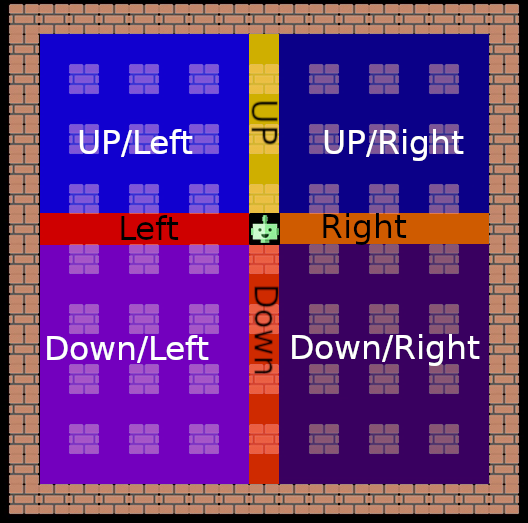
\includegraphics[width=\columnwidth]{Maze.png} % alternativ z.B. "width=6cm"
	\caption{Definition of the regions in the maze.}%
	\label{fig:Regions}%
\end{figure}

\subsubsection{Normalized potential rewards}

We show the regions regarding the second set, which make up the state. Each element, have the \textit{normalized potential rewards}(NPR) in each region, by mean of the $\omega_{R_{*}}$. And the weights $\omega_{R_{*}}$, are elements to measure  the potential reward to acquire, in all those eight regions described in figure \ref{fig:Regions}.

\begin{center}
\captionof{table}{How looks like the second array. Where the $\omega_{R_{*}}$ is the weight related to the NPR in each region.}
  \begin{tabular}{|c|}
\hline
Second array of the state: \\
\hline
$(\omega_{R_{U}},\omega_{R_{D}},\omega_{R_{L}},\omega_{R_{R}},\omega_{R_{UL}},\omega_{R_{DL}},\omega_{R_{DR}},\omega_{R_{UR}})$ \\
\hline
  \end{tabular}
  \label{table:S2}
\end{center}

Where:
\begin{equation}
    \omega_{R_*} \in [0,1]
\end{equation}


\subsubsection{Normalized potential danger}

The third set, is similar to the second one. 
Each element takes into acount the \textit{ Normalized Potential Danger }(NPD) in each region. And each weights $\omega_{D_{*}}$, is a measure of the potential danger in all those eigth regions.

Similary to the table \ref{table:S2}, we show how looks like the \textbf{NPD} float array.
\begin{center}
\captionof{table}{How looks like the second array. Where the $\omega_{R_{D_*}}$ is the weight related to the \textbf{NPD} in each region.}
  \begin{tabular}{|c|}
\hline
How looks like the second array of the state: \\
\hline
$(\omega_{D_{U}},\omega_{D_{D}},\omega_{D_{L}},\omega_{D_{R}},\omega_{D_{UL}},\omega_{D_{DL}},\omega_{D_{DR}},\omega_{D_{UR}})$ \\
\hline
  \end{tabular}
  \label{table:S3}
\end{center}


Where:
\begin{equation}
    \omega_{R_*} \in [0,1]
\end{equation}

\subsubsection{Drop a bomb (DB): Feasibility and usefulness}

To complete the state, we additionally add an array of two float values, regarding the situations where is feasible and useful to drop a bomb. The first value is a measure of the surrounding situation with the crates, and the second value is a measure of the proximity  of the opponents.

\begin{center}
\captionof{table}{How looks like the third array. Where the $\omega_{R_{D_Cr}}$ is the weight that measure the usefulness to get coins by blowing up crates, and $\omega_{R_{D_O}}$ the feasible of killing an opponent}
  \begin{tabular}{|c|}
\hline
How looks like the fourth array of the state: \\
\hline
$(\omega_{B_{Cr}},\omega_{B_{O}})$ \\
\hline
  \end{tabular}
  \label{table:S4}
\end{center}

Where:
\begin{equation}
    \omega_{B_*} \in [0,1]
\end{equation}

\subsubsection{Summary of state components}

In order to summarise the construct of the state, we describe the features selected. Which is made up of the four arrays shown in tables \ref{table:S1},\ref{table:S2},\ref{table:S3} and \ref{table:S4}:

\begin{table*}[t]
\centering
\captionof{table}{State summarized: Unsuccessfully attempt}
    \begin{tabular}{|l||c|c|c|r|}
     \hline
     \textbf{Abbreviation} & Description & Elements & Info & Type \\
     \hline
     \textbf{ACA}   &  Avalible cells & 4 & Directions & boolean \\
     \textbf{NPR}   &  Potential rewards & 8 & Regions & float  \\
     \textbf{NPD}   &  Potential danger & 8 & Regions & float  \\
     \textbf{DB}   &  Feasibility of throwing a bomb & 4 & Info crates and opponents & float  \\
     \hline
    \end{tabular}
    \label{table:S}
\end{table*}

\subsection{Second attempt: Simplifying the state}
\label{section:SimNRP}
In order to avoid correlated features, and achieve a functional version to complete the task 1 (\ref{section:Task1}). We simplify the NPR, in a binary version. 

The new NPR array is made up by four Booleans, where we calculate the nearest coin direction to operate the ACA with. 

\begin{figure}[t]% "t" = oben auf der Seite. Alternativ "b" f�r unten, "H" f�r direkt im Text
\centering	

	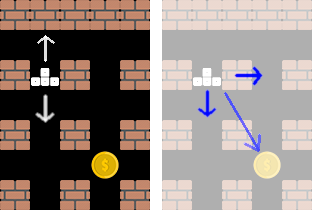
\includegraphics[width=\columnwidth]{NPR-1.png} % alternativ z.B. "width=6cm"
	\caption{Example of state formation, of ACA and NPR simplified: In the left side the avalible moves is showed, then ACA is: (1100), and in the right side, the direction of probable reward (DPR), and is given by: (0101). 
	from operate with the $\land$ operator, we get the $NPR = (1100)\land (0101)=(0100)$ }%
	\label{fig:NPREx}%
\end{figure}

Using the \textit{AND} operator $\land$. We construct the \textit{NPR} array, a picted example is showed in figure \ref{fig:NPREx}. And in case of $ACA\land DPR=(0,0,0,0)$, we chose randomly the \textit{NPR} form the composed \textit{ACA} possibilities

\subsection{Rewards}
The rewards for the agent should be evolutionary, that means, in principle the agent should learn to break the state of stillness, then it should acquire the capacity to move, then dropp bombs, survive the bombs that it has dropped, collect the coins it has found and finally fight against its opponents. In this process the rewards play an important role. For example at the beggining the reward of "WAITED" should be negative to encourage the agent to move. 
The following rewards were set:

        $OPPONENT\_ELIMINATED = 500$: this is a natural coice since the reward in the game is 5 and we scalate all the rewards by 100.
 \newline
        $COIN\_COLLECTED = 100$: another simple choice for the same reason that the opponent eliminated.
 \newline
        $CRATE\_DESTROYED = p_{foun\_coin}*COIN\_COLLECTED$, where $p_{foun\_coin}$ is the probabylity of found a coin taking into a account the number of crates at the begginig of the game.
 \newline
        $INVALID\_ACTION = -8$: this reward is negative to discourage the agent to take invalid actions.
 \newline
        $VALID = -2$: this reward make the agent take the shortest path, but in practice was useful just for the first task.
 \newline
        $COIN\_FOUND = 50$: this reward turned to be irrelevant due the actions that make it happen are already rewarded which are destroy crates and survive.
 \newline
        $KILLED\_SELF = -50$: this reward was the most difficult to tun, due one can think that should be pretty negative since die is sometihing quite undesired, but for training should be tuned carefully with smaller values, beacuse at the begginign, if the agent receives very negative reward for dying, that encourages the agent to don't dropp bombs because it get killed taking random actions, and therefore the agent can not continue with the evolutionary wanted process.
        $CRATE\_DESTROYED\_LESS = 4$: this reward is for the begginig of the training and it allows the agent to want to dropp bombs even if get killed but destroying a crate, which stimulate the agent to dropp bombs in correct places. Then the agent obtain $CRATE\_DESTROYED$ reward once it sucessfully destroyed a crate and survive, which is one of the most important behaviors the agent should learn.
        $WAIT = -2$: this reward is rather outstanding because is like the starter to all the evolutionary process, since it encourages the agent to do something and start learning. We found that even not setting this reward as negative the agent could arrive a good solution but slower.

\section{Training process}

\subsection{Action selection strategy for exploration}

The strategy used for exploration was $ \epsilon-greedy$. In this approach  the agent chooses what it believes to be the optimal action most of the time, but occasionally acts randomly. At the start of the training process the $\epsilon$ value is often initialized to a large probability, to encourage exploration in the face of knowing little about the environment. The value is then annealed down to a small constant (often 0.1), as the agent is assumed to learn most of what it needs about the environment \cite{PageStrategySelection}. 

We utilized this stratey because is rather straightforward to implement and it shows good resuts according to the community, thought we did not have time to experiment with any other strategy for exploration.

In the training we set the initial value of $\epsilon$ to $1$ and then decreases until $0.1$. We did not train with other values, again because lack of time.

\subsection{Hyperparameters for Deep Q-Learning}

We used the following hyperparameters for DQL:

As discount factor we used $\gamma = 0.95$ most of the time and $\gamma = 0.99$, showing similar results, this is because we weighted the future events almost as much as the instant ones.

The following hyperparameters were tuned based on several implementations of deep Q learning we looked at and based on the length of the state.

$memory\_size = 200000$: this is number of tuples $(state, action, reward, next state, done)$, where all are described by its name except for done, which indicates if an episode has ended. 

$replay\_minimun\_size = 1000$: this tells how many tuples we need to start to do the training, which is done at the end of each episode.

$batch\_size = 1000$: it indicates how many samples we get from the memory to propagated through the network .

$exploration\_steps = 100000$: it denotes the number of steps for which the $\epsilon$ is greater than $epsilon\_min = 0.1$, wich tells us the lower boundary of $\epsilon$ for the action selection strategy.

\section{Experimental Results}
\subsection{Task 1:}
\label{section:Task1}

{\it On a game board without any crates, collect a number of revealed coins as quickly as possible.
This task does not require dropping any bombs. The agent should learn how to navigate the
board effciently.}


For this task we use the state made up by the \textbf{ACA} array (see section \ref{section:ACA}) and the simplified \textbf{NRP} (see second \ref{section:SimNRP}). Summarised by the table \ref{table:Attemp2}.

\begin{table*}[!htbp]
\centering
\captionof{table}{State summarized}
    \begin{tabular}{|l||c|c|c|r|}
     \hline
     \textbf{Abbreviation} & Description & Elements & Info & Type \\
     \hline
     \textbf{ACA}   &  Avalible cells & 4 & Directions & Boolean \\
     \textbf{NPR simplified}   &  Nearest coin  & 4 & Directions & Boolean  \\
     \hline
    \end{tabular}
    \label{table:Attemp2}
\end{table*}

For this task, the agent must to learn two diferent skills. The fisrt one, is the skill to avoid the invalid actions, and the second one is to chose effciently the path to the coins. 

With the aim to kwon the learning evolution of the training, we calculate the total reward accumulated in all the training realization. At the begining of the training the amount of random actions predominate and the total reward accumulated start to decrease, later at the 150 episode, the agent will perform beter actions, and get positive rewards. Then, the total reward accumulated increase. See figure \ref{fig:TRewAccu}.

This behavior becomes clarified by mean of the figure \ref{fig:TRewAll}. Were shows, a convergence tendence after episode $400$. Up to get a maximal rewarded performed of $828$ (green)

In order to measure those skills, we show \cite{paperDQL}

\begin{figure}[t]% "t" = oben auf der Seite. Alternativ "b" f�r unten, "H" f�r direkt im Text
	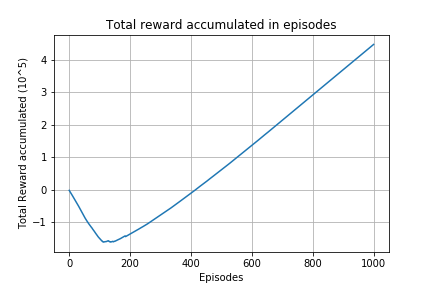
\includegraphics[width=\columnwidth]{TRewAccu.png} % alternativ z.B. "width=6cm"
	\caption{Total reward accumulated in episodes}%
	\label{fig:TRewAccu}%
\end{figure}

\begin{figure}[t]% "t" = oben auf der Seite. Alternativ "b" f�r unten, "H" f�r direkt im Text
	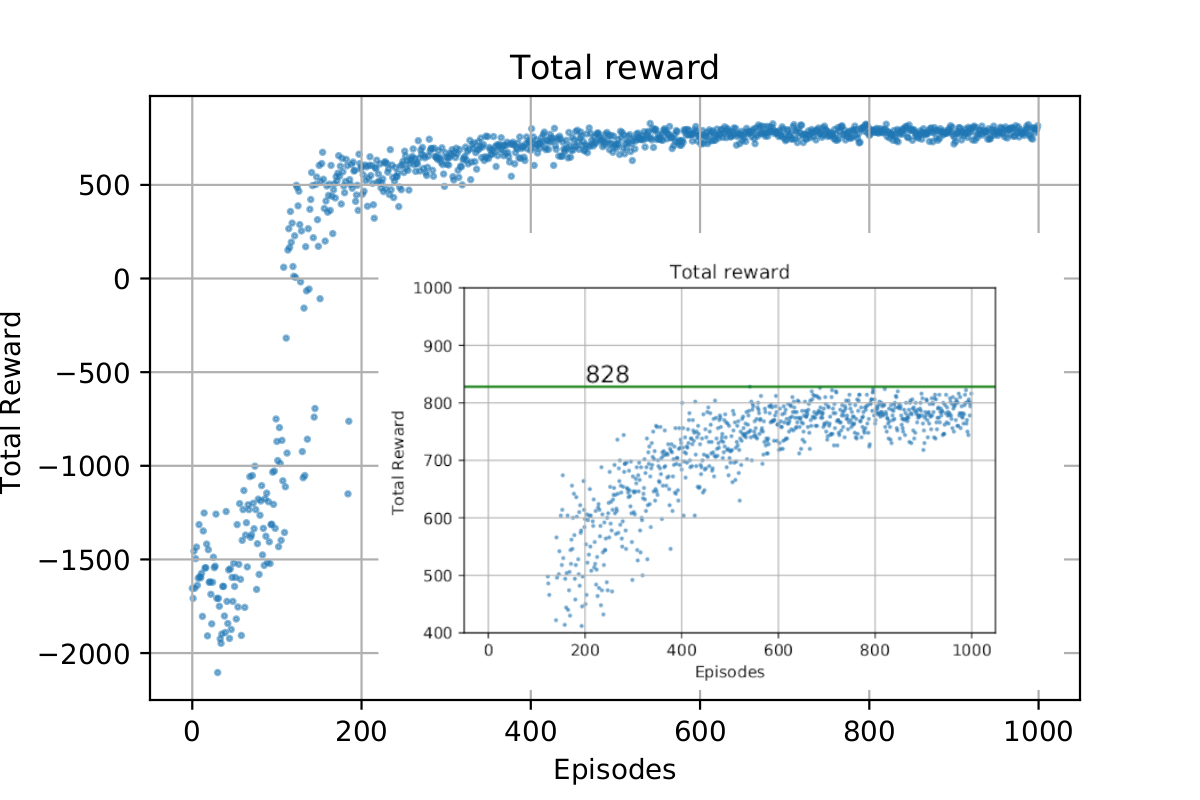
\includegraphics[width=\columnwidth]{TRewAll.png} % alternativ z.B. "width=6cm"
	\caption{Total reward in episodes. Plot inside: detailed behavior (in order to show the total reward tendence))}%
	\label{fig:TRewAll}%

\end{figure}

\begin{figure}[t]% "t" = oben auf der Seite. Alternativ "b" f�r unten, "H" f�r direkt im Text
	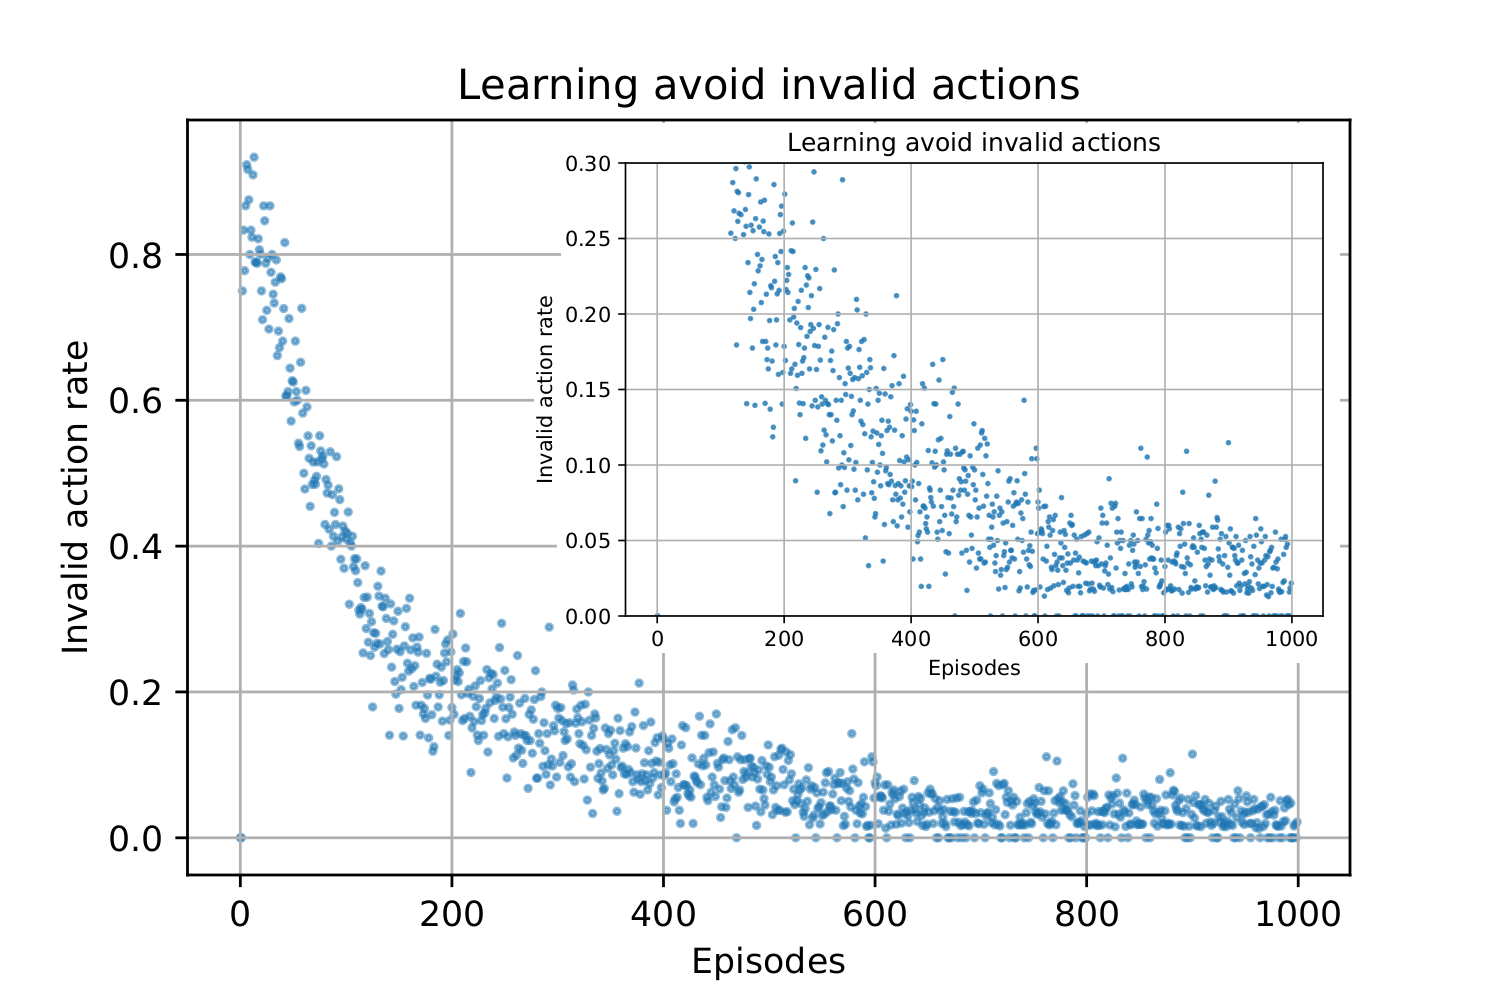
\includegraphics[width=\columnwidth]{Meassure1Coins.png} % alternativ z.B. "width=6cm"
	\caption{Meassuring the learning to avoid invalid actions. Plot inside: detailed behavior (in order to show the xtendence))}%
	\label{fig:M1Coins}%
\end{figure}


\begin{figure}[t]% "t" = oben auf der Seite. Alternativ "b" f�r unten, "H" f�r direkt im Text
	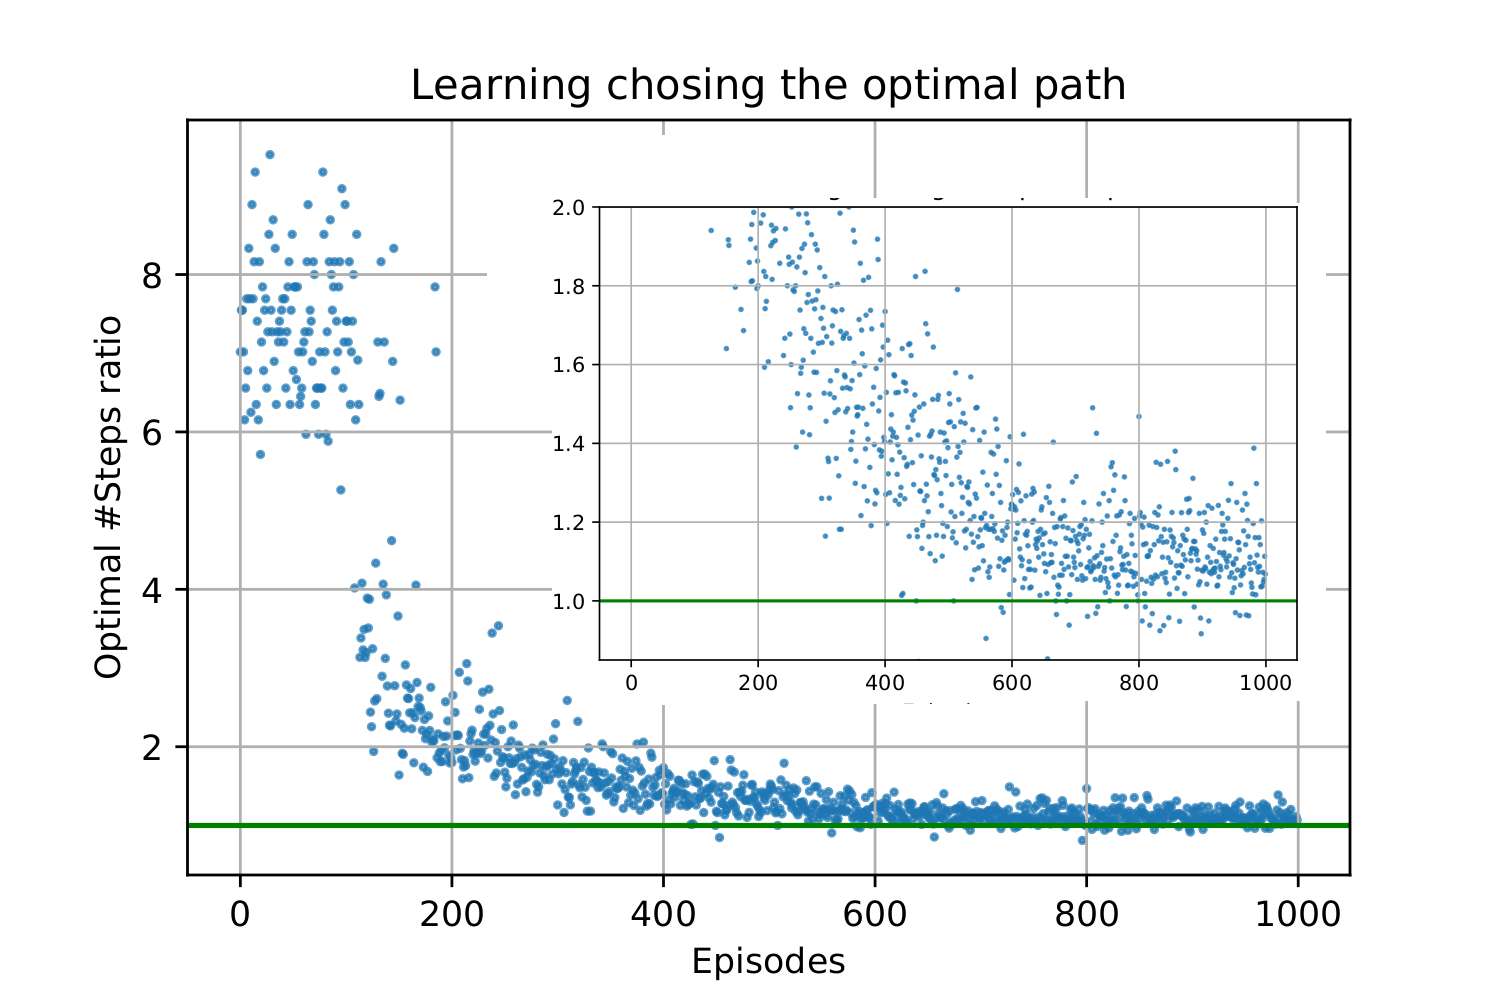
\includegraphics[width=\columnwidth]{Meassure2Coins.png} % alternativ z.B. "width=6cm"
	\caption{Meassuring the learning find the optimal path to get the coins. Plot inside: detailed behavior (in order to show the tendence))}%
	\label{fig:M1Coins}%
	
\end{figure}

\begin{figure}[t]% "t" = oben auf der Seite. Alternativ "b" f�r unten, "H" f�r direkt im Text
	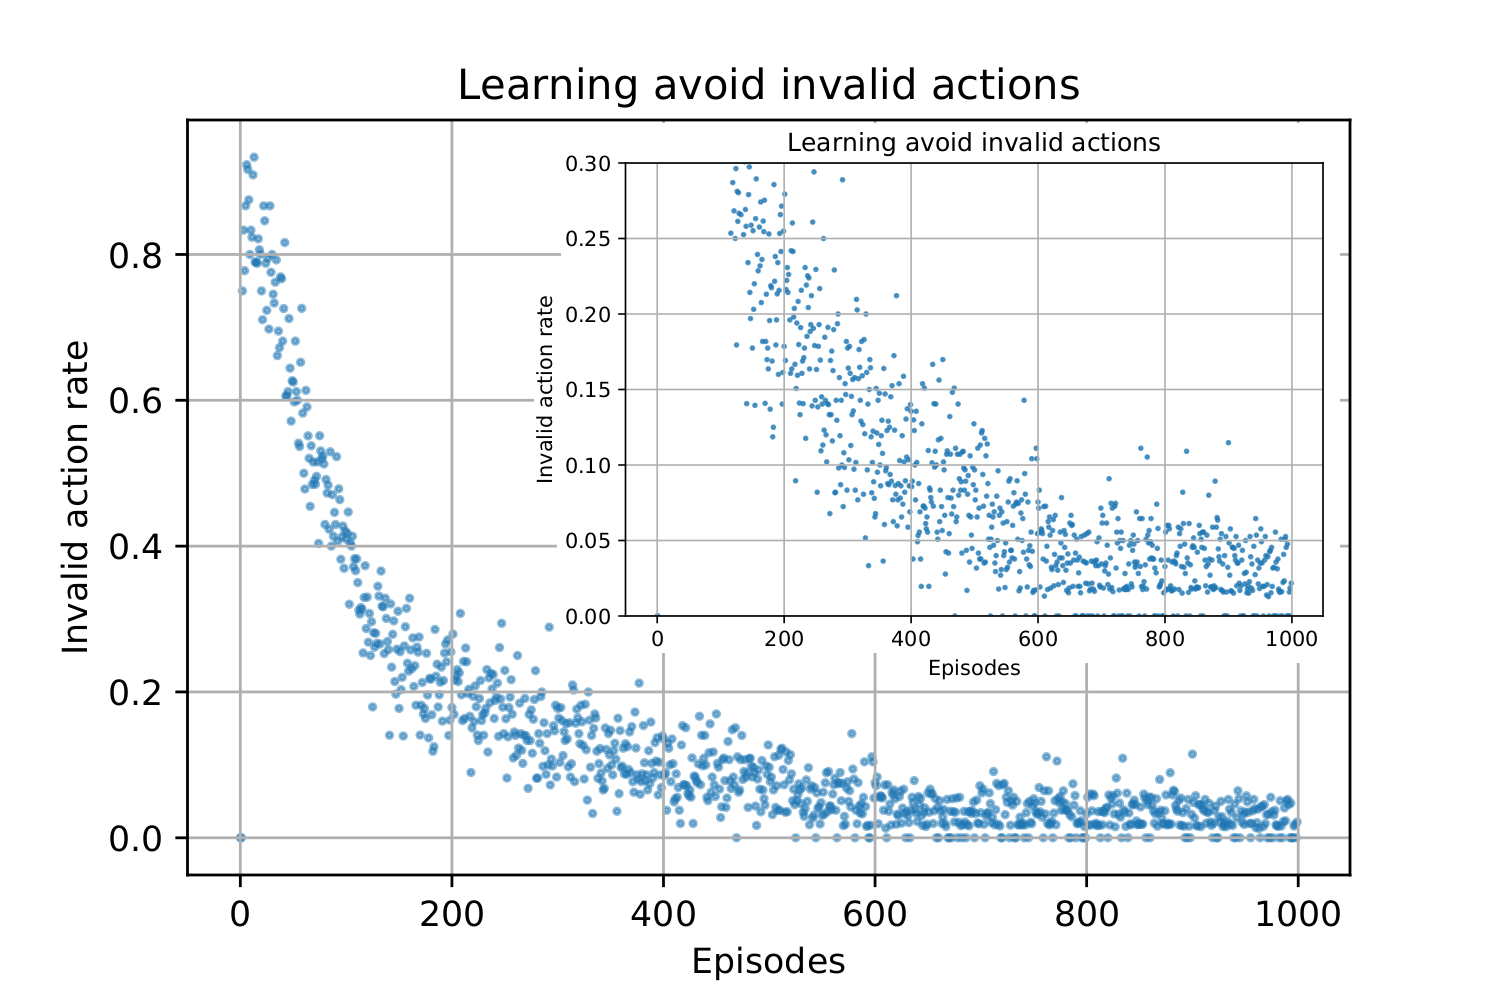
\includegraphics[width=\columnwidth]{Meassure1Coins.png} % alternativ z.B. "width=6cm"
	\caption{Meassuring the learning to avoid invalid actions. Plot inside: detailed behavior (in order to show the tendence))}%
	\label{fig:M1Coins}%
\end{figure}

\subsection{Task 2:}
{\it On a game board with randomly placed crates, find all hidden coins and collect them within the step limit. The agent must drop bombs to destroy the crates. It should learn how to use
bombs without killing itself, while not forgetting eficient navigation.} 

We tried to face the task 2 with the same strategy, but the problem was that when we performed the AND operator over the  $ACA$ and $DPR$ the result could be $(0, 0, 0, 0)$, because the nearest coin could be in a region where the direction was blocked, which again caused that the model did not converge to a desired result. 

We solved this problem by means of getting the nearest coin with respect to an unblocked direction and redefining $DPR$ by turning on the bit in this direction.

Another problem we found when solving the task 2 was that we could not punish too much the action of killed by itself, because  since the agent could die by dropping a bomb the agent avoided that action, which leaded to a situation where the agent survive the entire episode but without collecting any coin. So we decided to does not punish the action of killed by itself.


\section{Improving the agent and feedback}

\subsection{Improving the agent}
We learned many things in the development of the project,
among the most important ones are, try the easy solutions first and make sure that these approches work, then continue adding more complicated situations little by little, model them, and make sure that nothing is broken, because we discarded the simple solutions without even proving that they worked and when we tested the implementation of the complicated models and these didn't work we returned to previous ideas.
 
The agent could improve its results if we would have run it  in a GPU, this would have accelerated the tests and made everything faster. We thought that the time invested in setting up the GPU for the code could be potentially used for the design and the implementation, when we realized the slowleness of the trainign process was too late, though we think this is a common error of beginners.



\subsection{Feedback}

When we were training the model we realized that it could be handy to have the possibility to send parameters in the main to the program to speed up the the set up of the hyperparameters.

Another thing that could be handy is that was possible to get the remaining time that an opponent has to get a bomb again.

Another thing that could be improved is to have one not toy but easy example in the assigments or in the class to have a better understanding about the designing of the states, because we were pretty lost with this part at the begginig of the project.




\subsection{Q-learning with regression forest prediction}




\subsection{Neural Networks}

\subsection{General definitions:}

\subsubsection{Epsilon decay}
The exploration rate is defined by mena of the follow parameters:
\begin{lstlisting}
// Code
    #Initial exploration rate when training
    self.epsilon = 1.0
    # Exploration steps
    self.exploration_steps = 2000000
    # Minimum value of epsilon, after this value
    # epsilon does not decrease anymore
    self.epsilon_min = 0.1
    # This hyperparameter is to decrease the number
    # of explorations as the agent gets better
    self.epsilon_decay = (self.epsilon - self.epsilon_min) / self.exploration_steps
\end{lstlisting}

Then the \textit{exploration\_steps} is the parameter to fit in each realization. 
Were \textit{epsilon} decrease by \textit{self.epsilon $-=$ self.epsilon\_decay} with every step. 


\section{Motivation and overview}



\section{Model}
We basically tried to use 2 models, the normal Q learning and the deep Q learning. 
The model used for the training was constructed based on the algorithm known as Deep Q Learning \cite{paperDQL}


\subsection{Algorithm Deep Q Learning}


\begin{lstlisting}
// Code
    stringToMatch = 'Score'
    matchedLine = ''
    
    listScore = []
    listPasos = []
    listEpsil = []
    listRewaA = []
    listQMean = []

\end{lstlisting}




